\documentclass[11pt,a4paper]{article}

\usepackage[utf8]{inputenc}
\usepackage[T1]{fontenc}
\usepackage{lmodern}
\usepackage[margin=2.4cm]{geometry}
\usepackage{amsmath,amssymb}
\usepackage{booktabs}
\usepackage{graphicx}
\usepackage{longtable}
\usepackage{array}
\usepackage{xcolor}
\usepackage{microtype}
\usepackage[hidelinks]{hyperref}
\usepackage{caption}
\usepackage{enumitem}
\usepackage{fancyhdr}
\usepackage{float}

\definecolor{measured}{RGB}{54,83,20}
\definecolor{risk}{RGB}{127,29,29}
\newcommand{\meas}{\textcolor{measured}{\textbf{[measured]}}}

\pagestyle{fancy}
\fancyhf{}
\lhead{\small PHAROS: A Physics-Grounded MoE Architecture for RNA Structure}
\rhead{\small\thepage}
\renewcommand{\headrulewidth}{0.4pt}

\title{\textbf{PHAROS}\\[0.3em]
\large A Physics-Hybrid, Attention-Routed Mixture-of-Experts Architecture\\
for RNA Structure and Contact-Map Prediction\\[0.6em]
\normalsize Architecture Design Report --- Version 0.1}
\author{Shuvam Banerji Seal\\\small SBS-RNA Project}
\date{12 September 2026}

\begin{document}
\maketitle

\begin{abstract}
\noindent
RNA three-dimensional structure prediction has not had its AlphaFold2 moment.
The best current methods reach a mean TM-score of approximately $0.55$ on
non-redundant benchmarks, which is the threshold for recovering roughly the
correct fold, against routine scores above $0.9$ for proteins. This report
argues that the bottleneck is not model scale but \emph{inductive bias}, and
specifies an architecture, \textbf{PHAROS}, built around that claim.

Three empirical findings drive the design. First, ERNIE-RNA (86M parameters)
outperforms RiNALMo (650M) and UNI-RNA (400M) on secondary-structure prediction,
and nearly doubles cross-family generalisation relative to RiNALMo ($F_1 = 0.646$
versus $0.355$), on the strength of a single hand-set, three-valued base-pairing
prior added to its attention logits. Second, we measure on 117 non-redundant RNA
chains that contacts per nucleotide \emph{saturates} at $4.4$--$4.9$ while
contact-map density falls from $6.5\%$ at $L \approx 56$ to $0.353\%$ at
$L \approx 2900$: RNA contact maps scale as $O(L)$, not $O(L^2)$, so a dense
pair representation spends over $99\%$ of its compute on empty space and would
require $309$~GB of activations at $L=2048$. Third, we measure a monotonic
$1.76\sigma$ gradient in normalised crystallographic B-factor as a function of
distance to the nearest $\mathrm{Mg}^{2+}$ ion across $24{,}623$ nucleotides,
establishing that ion coordination and local rigidity are not independent
features but two readouts of one phenomenon.

PHAROS accordingly (i) accepts \textbf{ionic conditions as a model input},
which no existing RNA structure predictor does, propagating them to attention
logits through a Manning-renormalised screened-Coulomb bias---though an audit
reported here shows the \emph{learned} part of that claim cannot be trained on
the PDB, whose recorded Mg\textsuperscript{2+} spans only 5--15 mM because
nobody deposits unfolded RNA; (ii) replaces the
dense pair track with a \textbf{hierarchical coarse-to-fine pair track} that
selects contact-bearing \emph{blocks} rather than pairs, at $2.2\%$ of dense
cost---adopted after we measured a flat top-$K$ design recovering only
\emph{one contact in five} on long chains, and measured block occupancy falling
to $1.34\%$ as chains lengthen; (iii) routes a \textbf{sparse
mixture-of-experts} on local structural regime rather than sequence context,
supported by our negative result that GNRA $k$-mer context predicts rigidity at
only $0.073\sigma$; and (iv) supplies motif geometry through a \textbf{frozen
retrieval bank} of 667 RNA 3D Motif Atlas classes rather than expecting the
model to learn it from 6{,}661 structurally-resolved sequences. We also identify
two supervision channels---$\mathrm{Mg}^{2+}$ sites and B-factor
rigidity---that are already present in every mmCIF file the field downloads and
are currently used by no structure predictor.

This is a design specification. No model has been trained. All quantitative
claims are either marked \meas{} and reproducible from the scripts in this
repository, or cited to the literature.
\end{abstract}

\tableofcontents
\newpage

%========================================================
\section{Problem statement}

\subsection{The accuracy gap}

Table~\ref{tab:sota} gives the state of the art on a non-redundant RNA test set
as of November 2025.

\begin{table}[h]
\centering
\caption{Current state of the art in RNA 3D structure prediction.}
\label{tab:sota}
\begin{tabular}{lcl}
\toprule
\textbf{Method} & \textbf{Mean TM-score} & \textbf{Approach} \\
\midrule
trRosettaRNA   & $\mathbf{0.548}$ & MSA $\rightarrow$ restraints $\rightarrow$ folding \\
NuFold         & $0.525$ & AlphaFold2-style nucleotide frames \\
AlphaFold3 (server) & $0.510$ & all-atom diffusion \\
AlphaFold3 (local)  & $0.504$ & all-atom diffusion \\
\bottomrule
\end{tabular}
\end{table}

A TM-score near $0.5$ means the topology is approximately right and little else.
The CASP16 signal is equally instructive: leading RNA groups won by integrating
AlphaFold3 \emph{into physics-based modelling} rather than by scaling a neural
network. Physics-plus-machine-learning hybrids are currently ahead in RNA,
which is the premise this architecture is built on.

\subsection{Why RNA lags}

\begin{enumerate}[leftmargin=1.4em,itemsep=0.2em]
\item \textbf{Data scarcity.} Our catalogue records $6{,}661$ unique sequences
with experimental 3D structure against $1.37$ billion sequences, a coverage of
$0.0005\%$. Proteins had roughly $220{,}000$ structures at the AlphaFold2
moment.
\item \textbf{Redundancy within that data.} $15{,}441$ RNA3DB chains collapse to
$3{,}157$ unique sequences; 5S rRNA alone accounts for $5{,}976$ BGSU
equivalence classes.
\item \textbf{Family coverage.} Only $100$ of $4{,}227$ Rfam families ($2.4\%$)
have any 3D representative.
\item \textbf{Conformational plasticity.} Riboswitches are \emph{defined} by
adopting multiple functional folds; single-structure prediction is the wrong
target for a large fraction of functional RNA.
\item \textbf{Ion dependence.} RNA is a polyanion. Its fold is not defined
without specifying the ionic environment, yet no mainstream predictor accepts
ionic conditions as an input.
\item \textbf{Target noise.} Median resolution in our catalogue is $3.10$~\AA{},
with only $13\%$ of chains at $2.5$~\AA{} or better.
\end{enumerate}

%========================================================
\section{The central argument: bias beats scale}

Table~\ref{tab:ernie} contains the most important result in the recent RNA
language-model literature.

\begin{table}[h]
\centering
\caption{ERNIE-RNA versus larger dense models. A 7.5$\times$ parameter deficit
is overturned by one hand-set prior.}
\label{tab:ernie}
\begin{tabular}{lccc}
\toprule
\textbf{Model} & \textbf{Params} & \textbf{bpRNA-1m $F_1$} & \textbf{bpRNA-new $F_1$} \\
\midrule
ERNIE-RNA (attention map) & 86M  & $\mathbf{0.873}$ & --- \\
ERNIE-RNA (embedding)     & 86M  & $0.862$ & $\mathbf{0.646}$ \\
RiNALMo                   & 650M & $0.850$ & $0.355$ \\
UNI-RNA                   & 400M & $0.821$ & --- \\
RNA-FM                    & 100M & $0.808$ & --- \\
\bottomrule
\end{tabular}
\end{table}

ERNIE-RNA's entire architectural advantage is an additive bias on attention
logits. In its first layer,
\begin{equation}
\mathrm{Attention}(Q,K) = \frac{QK^{\top}}{\sqrt{d}} + B_{\text{pair}}(i,j),
\qquad
\mathrm{Attention}_{l}(Q,K) = \frac{QK^{\top}}{\sqrt{d}} + \mathrm{Attention}_{l-1}(Q,K),
\end{equation}
with $B_{\text{pair}}$ set by hand to $3$ for C--G, $2$ for A--U, a tunable
$\alpha \approx 0.8$ for G--U, and $0$ on the diagonal.

The cross-family result is the decisive one: $0.646$ versus $0.355$. A fixed
physical prior nearly doubles generalisation to unseen families, because the
prior is true regardless of family whereas learned family statistics are not.

\begin{quote}
\textbf{Thesis.} If a crude three-valued prior buys more than $7\times$ the
parameters, the marginal return on \emph{better physics} exceeds the marginal
return on \emph{more scale}. PHAROS replaces that hand-set prior with a learned,
ion-aware, motif-aware, coevolution-aware one.
\end{quote}

Its limitations define our openings. The prior is static, so a G--U pair inside
a kink-turn is treated identically to one in a free helix. It is
nearest-neighbour-blind, whereas real pairing energy is stacking-dependent. It
encodes only canonical pairing, while non-canonical pairs define RNA 3D motifs
and carry most tertiary information. And it ignores ions entirely.

%========================================================
\section{Empirical analysis}

All results in this section were measured for this report on 180 BGSU
non-redundant representative structures at $\leq 3.0$~\AA{}, downloaded and
analysed by scripts in \texttt{.../sampling/}. Raw outputs are in
\texttt{data/samples/analysis/}.

\subsection{RNA contact maps scale linearly, not quadratically}

Contacts are defined as nucleotide pairs with any heavy-atom pair within
$8.0$~\AA{} and sequence separation $|i-j| \geq 4$.

\begin{table}[h]
\centering
\caption{Contact density by chain length across 117 chains. \meas}
\label{tab:sparsity}
\begin{tabular}{lcccc}
\toprule
\textbf{Chain length} & \textbf{$n$} & \textbf{median $L$} & \textbf{contacts/nt} & \textbf{map density} \\
\midrule
32--100    & 38 & 56   & $1.784$ & $6.523\%$ \\
100--200   & 6  & 124  & $2.851$ & $4.043\%$ \\
200--500   & 3  & 393  & $4.216$ & $2.151\%$ \\
500--1500  & 9  & 1038 & $4.532$ & $0.974\%$ \\
$\geq 1500$ & 61 & 2901 & $4.854$ & $\mathbf{0.353\%}$ \\
\midrule
\multicolumn{2}{l}{\textbf{Overall}} & & median $4.397$, p95 $5.422$, max $5.497$ & median $0.389\%$ \\
\bottomrule
\end{tabular}
\end{table}

Contacts per nucleotide saturates at $4.4$--$4.9$ and is bounded by RNA
coordination geometry, independent of length; density falls approximately as
$1/L$. The number of contacts therefore grows \emph{linearly} in $L$.

The consequence for architecture is immediate. A dense pair representation of
dimension $c=128$ requires, for 48 blocks holding roughly six intermediate
tensors each and without gradient checkpointing:
\[
L=512 \rightarrow 19.3~\text{GB}, \qquad
L=1024 \rightarrow 77.3~\text{GB}, \qquad
L=2048 \rightarrow 309.2~\text{GB}.
\]
A dense pair track is not merely wasteful at RNA lengths; it is infeasible.
How that sparsity is exploited turns out to matter as much as exploiting it at
all: a flat top-$K$ selection fails on long chains, and contacts must be
selected as \emph{blocks}. Section~\ref{sec:hpt} reports both measurements.

\subsection{Ion coordination and local rigidity are one phenomenon}

We z-normalise crystallographic B-factors within each structure so that
refinement protocols are comparable, and restrict this analysis to the 31 X-ray
structures among the sample; cryo-EM atomic displacement parameters are not
comparable and were excluded. Lower $z_B$ indicates greater rigidity.

\begin{table}[h]
\centering
\caption{Normalised B-factor versus distance to the nearest $\mathrm{Mg}^{2+}$,
over $24{,}623$ nucleotides. \meas}
\label{tab:mgrigid}
\begin{tabular}{lcc}
\toprule
\textbf{Distance to nearest $\mathrm{Mg}^{2+}$} & \textbf{$n$ nucleotides} & \textbf{mean $z_B$} \\
\midrule
$0$--$4$~\AA{}    & 319   & $\mathbf{-0.883}$ \\
$4$--$6$~\AA{}    & 2{,}441 & $-0.673$ \\
$6$--$8$~\AA{}    & 7{,}590 & $-0.415$ \\
$8$--$12$~\AA{}   & 8{,}115 & $+0.004$ \\
$12$--$20$~\AA{}  & 2{,}984 & $+0.756$ \\
$> 20$~\AA{}      & 3{,}174 & $\mathbf{+0.877}$ \\
\bottomrule
\end{tabular}
\end{table}

The gradient is monotonic and spans $1.76$ standard deviations. Local packing
density independently correlates with rigidity at Pearson $r = -0.294$.

\begin{quote}
\textbf{Architectural consequence.} Ion effects and motif rigidity, which the
project brief treats as two separate physical ingredients, are strongly coupled.
A model that predicts $\mathrm{Mg}^{2+}$ sites obtains a rigidity map nearly for
free and vice versa. That mutual information justifies routing them into a
\emph{shared} physics expert rather than two disconnected heads.
\end{quote}

\paragraph{Caveats.} B-factor also absorbs resolution, occupancy and refinement
choices. $\mathrm{Mg}^{2+}$ proximity and dense packing are themselves
correlated, since both mark folded cores, so this is association rather than
isolated causation; the gradient partly restates that structured cores both bind
ions and are ordered. The closest bin contains only $319$ nucleotides. This is
strong evidence for \emph{using} the coupling as a prior, not a proof of
mechanism.

\subsection{Ion inventory and coordination chemistry}

\begin{table}[h]
\centering
\caption{Cation inventory across 179 parsed structures. \meas}
\label{tab:ions}
\begin{tabular}{lr@{\hskip 2em}lr}
\toprule
\textbf{Ion} & \textbf{Count} & \textbf{Inner-sphere partner} & \textbf{Count} \\
\midrule
$\mathrm{Mg}^{2+}$ & $\mathbf{17{,}428}$ & OP2 (phosphate) & 5{,}890 \\
$\mathrm{K}^{+}$   & 1{,}868 & OP1 (phosphate) & 5{,}144 \\
$\mathrm{Zn}^{2+}$ & 359   & O6 (guanine)    & 757 \\
$\mathrm{Na}^{+}$  & 161   & O4 (uracil)     & 511 \\
$\mathrm{Ca}^{2+}$ & 29    & N7 (purine)     & 447 \\
$\mathrm{Mn}^{2+}$ & 12    & O2$'$ (ribose)  & 196 \\
\bottomrule
\end{tabular}
\end{table}

$\mathrm{Mg}^{2+}$ outnumbers all other cations by roughly $9\!:\!1$, so an
ion-aware model that handles a single species should handle $\mathrm{Mg}^{2+}$.
Some $83\%$ of direct coordination is to the two non-bridging phosphate oxygens;
the next largest class, G(O6)/G(N7), is the textbook major-groove guanine site.

Coordination is predominantly water-mediated: a mean of $0.77$ inner-sphere
against $7.00$ outer-sphere RNA contacts per $\mathrm{Mg}^{2+}$. Crucially the
inner-sphere fraction is itself a function of tertiary compactness: $0.511$
overall but only $0.296$ for chains shorter than $500$~nt. The inner/outer ratio
is therefore a \emph{predictable readout} of compactness, not merely an input.

\paragraph{Stratification warning.} These aggregates are ribosome-dominated and
must not be quoted flat. The five largest structures hold $39.4\%$ of all
$\mathrm{Mg}^{2+}$. Per structure the median is $72.5$ ions against a mean of
$181.5$; per nucleotide the median is $0.046$, roughly one $\mathrm{Mg}^{2+}$
per $22$ nucleotides.

\paragraph{What crystallography cannot see.} Resolved $\mathrm{Mg}^{2+}$ are
site-bound ions only. The diffuse Manning atmosphere, which neutralises roughly
$76\%$ of backbone charge, is invisible to crystallography. The two channels
must be modelled separately and never conflated.

\subsection{Coevolution is strong, but gated by alignment depth}
\label{sec:coev}

Coevolution is the oldest structural signal in the field: a base pair tolerates
mutation at one position only when compensated at the other, so paired columns
covary across a family alignment. We measured how much of that signal is
actually recoverable, computing sequence-reweighted, pseudocounted,
APC-corrected mutual information on the 12 downloaded Rfam seed alignments and
scoring it against each family's curated consensus secondary structure
(\texttt{\#=GC SS\_cons}), restricted to $|i-j| \geq 4$.

\begin{table}[h]
\centering
\caption{APC-corrected MI against curated consensus base pairs. \meas}
\label{tab:coev}
\small
\begin{tabular}{lrrrcc}
\toprule
\textbf{Family} & \textbf{$N$} & \textbf{$N_{\text{eff}}$} & \textbf{$L$} & \textbf{prec@$L/5$} & \textbf{rec@$L$} \\
\midrule
tRNA (RF00005)              & 954 & $245.9$ & 71  & $\mathbf{1.000}$ & $\mathbf{1.000}$ \\
THF riboswitch (RF01831)    & 101 & $27.9$  & 100 & $1.000$ & $0.906$ \\
Purine riboswitch (RF00167) & 133 & $102.7$ & 102 & $0.950$ & $0.955$ \\
5S rRNA (RF00001)           & 712 & $10.3$  & 119 & $0.826$ & $0.765$ \\
RNase P bacterial (RF00010) & 458 & $11.6$  & 367 & $0.753$ & $0.784$ \\
SAM riboswitch (RF00162)    & 457 & $19.9$  & 108 & $0.714$ & $0.697$ \\
Cobalamin (RF00174)         & 434 & $63.1$  & 189 & $0.676$ & $0.667$ \\
Glutamine (RF01739)         & 940 & $15.6$  & 53  & $0.500$ & $0.692$ \\
ydaO/yuaA (RF00379)         & 106 & $18.4$  & 134 & $0.462$ & $0.615$ \\
TPP riboswitch (RF00059)    & 115 & $41.3$  & 105 & $0.429$ & $0.926$ \\
tmRNA (RF00023)             & 477 & $74.6$  & 378 & $0.400$ & $0.670$ \\
FMN riboswitch (RF00050)    & 146 & $21.2$  & 139 & $0.333$ & $0.536$ \\
\midrule
\textbf{mean}               &     &         &     & $\mathbf{0.670}$ & $\mathbf{0.768}$ \\
\bottomrule
\end{tabular}
\end{table}

The decisive pattern is the depth dependence. Splitting on $N_{\text{eff}}/L$:
families at $N_{\text{eff}}/L \geq 1$ ($n=2$) reach mean precision@$L/5$ of
$\mathbf{0.975}$, while those below ($n=10$) reach $0.609$. tRNA, at
$N_{\text{eff}}/L = 3.5$, is perfect on both precision and recall.

Note how \emph{few} families are deep: only 2 of 12, and these are hand-curated
Rfam seed alignments, among the best-conditioned RNA alignments in existence.
Automatic homology search on an arbitrary sequence will generally do worse.

\begin{quote}
\textbf{Architectural consequence, and the strongest argument for MoE in this
design.} Coevolution is not a weak feature to be blended in at fixed weight---where
the alignment is deep it is very nearly sufficient on its own. But its
availability is conditional, and the condition $N_{\text{eff}}/L$ is
\emph{cheaply computable before the model runs}. The correct expert therefore
depends on an observable property of the input, which is exactly what a mixture
of experts is for. $N_{\text{eff}}/L$ becomes an explicit router feature, and
the coevolution expert is gated on it. This also explains why RhoFold+ pairs a
language model \emph{with} MSA features rather than choosing between them: the
two have complementary failure modes. PHAROS makes that complementarity routed
and explicit instead of concatenated.
\end{quote}

\paragraph{An implementation note worth recording.} A first version of this
measurement reported mean precision $0.039$. That was a defect, not a property
of RNA: the outer-product term in the MI normalisation broadcast to shape
$(C,q,1)$ rather than $(C,q,q)$, so only diagonal terms contributed. After
correcting it and adding standard DCA sequence reweighting at $80\%$ identity
with pseudocounts, precision rose seventeenfold to $0.670$. A plausible-looking
weak result was a silent bug.

\paragraph{Caveats.} The ground truth here is Rfam's consensus \emph{secondary}
structure, not 3D contacts, so this measures recovery of curated pairing rather
than direct tertiary contact accuracy. Twelve curated seed families is a small
and favourable sample. APC-corrected MI is also a simplification of full DCA;
pseudo-likelihood DCA would do better, so these values are a reasonable lower
bound on the available signal.

\subsection{A negative result that constrains the design}

We tested whether GNRA-like tetraloop sequence context alone predicts rigidity,
matching the 4-mers \{GAAA, GCAA, GAGA, GUGA, GGAA, GCGA, GUAA, GAAG\} anywhere
in a chain.

\begin{table}[h]
\centering
\caption{GNRA $k$-mer context versus rigidity. \meas{} Effect size $0.073\sigma$.}
\label{tab:gnra}
\begin{tabular}{lcc}
\toprule
\textbf{Context} & \textbf{$n$ nucleotides} & \textbf{mean $z_B$} \\
\midrule
GNRA-like 4-mer & 4{,}944 & $-0.082$ \\
All other       & 95{,}768 & $-0.009$ \\
\bottomrule
\end{tabular}
\end{table}

The effect is negligible. The likely cause is methodological: a GNRA
\emph{sequence} is a GNRA \emph{tetraloop} only when it actually caps a hairpin,
and linear 4-mer matching counts mostly helical and junction occurrences.

\begin{quote}
\textbf{Architectural consequence.} Sequence context alone does not identify a
motif. Motif identity requires the interaction graph. The motif machinery must
therefore be conditioned on the pair representation after secondary structure is
available, never on raw $k$-mers. This rules out the naive
``learn motifs from sequence $n$-grams'' design.
\end{quote}

%========================================================
\section{The PHAROS architecture}

\begin{figure}[h]
\centering
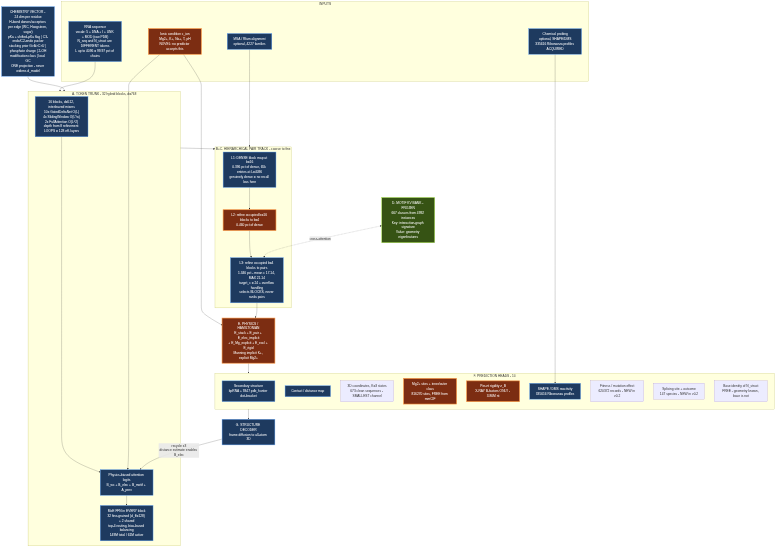
\includegraphics[width=0.86\textwidth,keepaspectratio]{../architecture/diagrams/rendered/01-system-overview.png}
\caption{PHAROS system overview. Orange denotes novel components, green denotes
frozen retrieval, blue denotes adapted standard components.}
\end{figure}

\subsection{Inputs}

\begin{table}[h]
\centering
\begin{tabular}{llp{6.5cm}}
\toprule
\textbf{Input} & \textbf{Required} & \textbf{Note} \\
\midrule
Sequence, $L$ tokens, vocab 5 & yes & elDORS is DNA-alphabet; $T \rightarrow U$ at load \\
Ionic condition $c_{\text{ion}}$ & yes, defaulted & $([\mathrm{Mg}^{2+}],[\mathrm{K}^{+}],[\mathrm{Na}^{+}],T,\mathrm{pH})$; \textbf{novel} \\
MSA / Rfam alignment & optional & graceful degradation when shallow \\
Chemical probing profile & optional & not yet acquired (Section~\ref{sec:gap}) \\
\bottomrule
\end{tabular}
\end{table}

Ionic condition enters as a FiLM-style conditioning vector, analogous to a
diffusion timestep embedding. The same sequence at $0$~mM and $10$~mM
$\mathrm{Mg}^{2+}$ must produce different predictions; this is the clearest
novelty claim in the design.

\subsection{Token trunk: hybrid attention with MoE}

\begin{figure}[p]
\centering
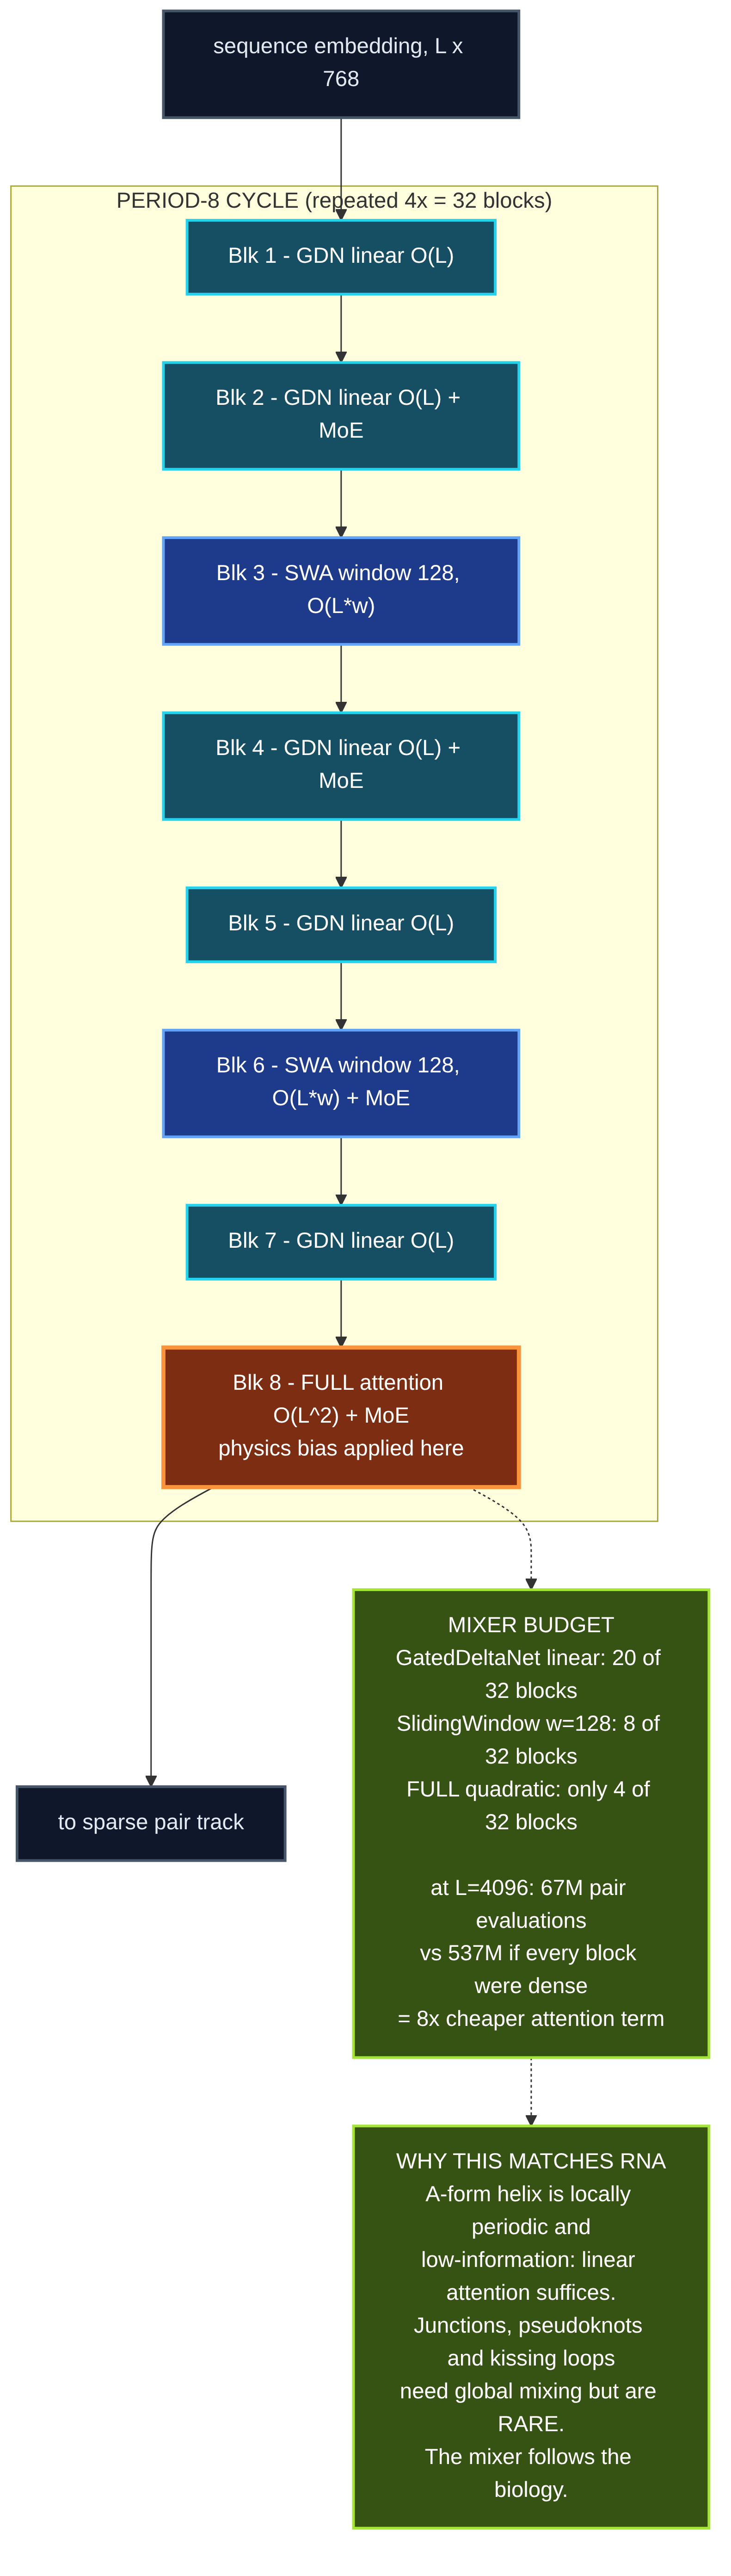
\includegraphics[height=0.82\textheight,keepaspectratio]{../architecture/diagrams/rendered/02-token-trunk.png}
\caption{Period-8 mixer interleaving, repeated four times for 32 blocks.}
\end{figure}

The trunk uses 32 blocks at $d=768$ with the repeating pattern
\[
[\,\mathrm{GDN},\ \mathrm{GDN},\ \mathrm{SWA},\ \mathrm{GDN},\ \mathrm{GDN},\ \mathrm{SWA},\ \mathrm{GDN},\ \mathrm{FULL}\,],
\]
where GDN is Gated DeltaNet linear attention ($O(L)$, 20 of 32 blocks), SWA is
sliding-window softmax attention with window 128 ($O(Lw)$, 8 blocks), and FULL
is full attention with physics bias ($O(L^2)$, only 4 blocks).

The justification is both architectural and biological. Jamba interleaves
Mamba, attention and MoE at a $7\!:\!1$ ratio and reaches 256K context with a
$4$~GB KV cache; Gated DeltaNet outperforms Mamba2 and DeltaNet on in-context
retrieval and length extrapolation; Oryx varies the mixer type \emph{within} a
sequence. RNA has exactly the structure this exploits: long stretches of regular
A-form helix that are locally periodic and low-information, punctuated by rare
junctions, pseudoknots and kissing loops that require global mixing. At
$L=4096$, an all-dense 32-block trunk would perform $537$M pair evaluations;
PHAROS performs $67$M, an $8\times$ reduction.

\subsubsection{Physics-biased attention}

In SWA and FULL blocks the attention logits carry four additive terms:
\begin{equation}
A_{ij} = \frac{Q_i K_j^{\top}}{\sqrt{d}}
       + B_{\mathrm{wc}}(i,j)
       + B_{\mathrm{elec}}(i,j;\,c_{\text{ion}})
       + B_{\mathrm{motif}}(i,j)
       + A^{(l-1)}_{ij}.
\end{equation}

$B_{\mathrm{wc}}$ generalises ERNIE-RNA's fixed prior to a learned pair-type
embedding modulated by stacking context, since real pairing energy is
nearest-neighbour dependent. It is initialised at the ERNIE-RNA values so
training begins from a known-good prior. The term $A^{(l-1)}$ retains
ERNIE-RNA's attention accumulation.

$B_{\mathrm{elec}}$ is the novel term. With Bjerrum length
$\ell_B = e^2/(4\pi\varepsilon_0\varepsilon_r k_B T) \approx 7.1$~\AA{} in water
at $298$~K, Manning parameter $\xi = \ell_B/b$ for axial charge spacing $b$,
condensed fraction and renormalised charge
\begin{equation}
\theta = 1 - \frac{1}{z\xi}, \qquad q_{\text{eff}} = -(1-\theta),
\end{equation}
and Debye screening parameter
$\kappa = \sqrt{2 N_A e^2 I / (\varepsilon\varepsilon_0 k_B T)}$ from ionic
strength $I$, the bias is
\begin{equation}
B_{\mathrm{elec}}(i,j) = -\lambda\, q_{\text{eff}}^{2}\, \ell_B\,
\frac{\exp(-\kappa d_{ij})}{d_{ij}}.
\label{eq:belec}
\end{equation}
For monovalent RNA $\theta \approx 0.76$, so roughly three quarters of backbone
charge is screened before any structure-specific electrostatics is considered.
Only $\lambda$ is learned; $q_{\text{eff}}$, $\kappa$ and $\ell_B$ follow in
closed form from $c_{\text{ion}}$ and temperature. Equation~\eqref{eq:belec} is
the mechanism by which salt concentration changes the prediction.

\paragraph{Resolving the circularity.} Equation~\eqref{eq:belec} requires
$d_{ij}$, which is unknown on the first pass. $B_{\mathrm{elec}}$ is therefore
disabled at recycle 0 and enabled from recycle 1 using the current predicted
distance map. Recycling is thus structural to the design rather than an
optimisation: the physics term needs a geometry estimate to evaluate, and each
recycle sharpens both.

\subsubsection{Mixture-of-experts feed-forward}

\begin{figure}[p]
\centering
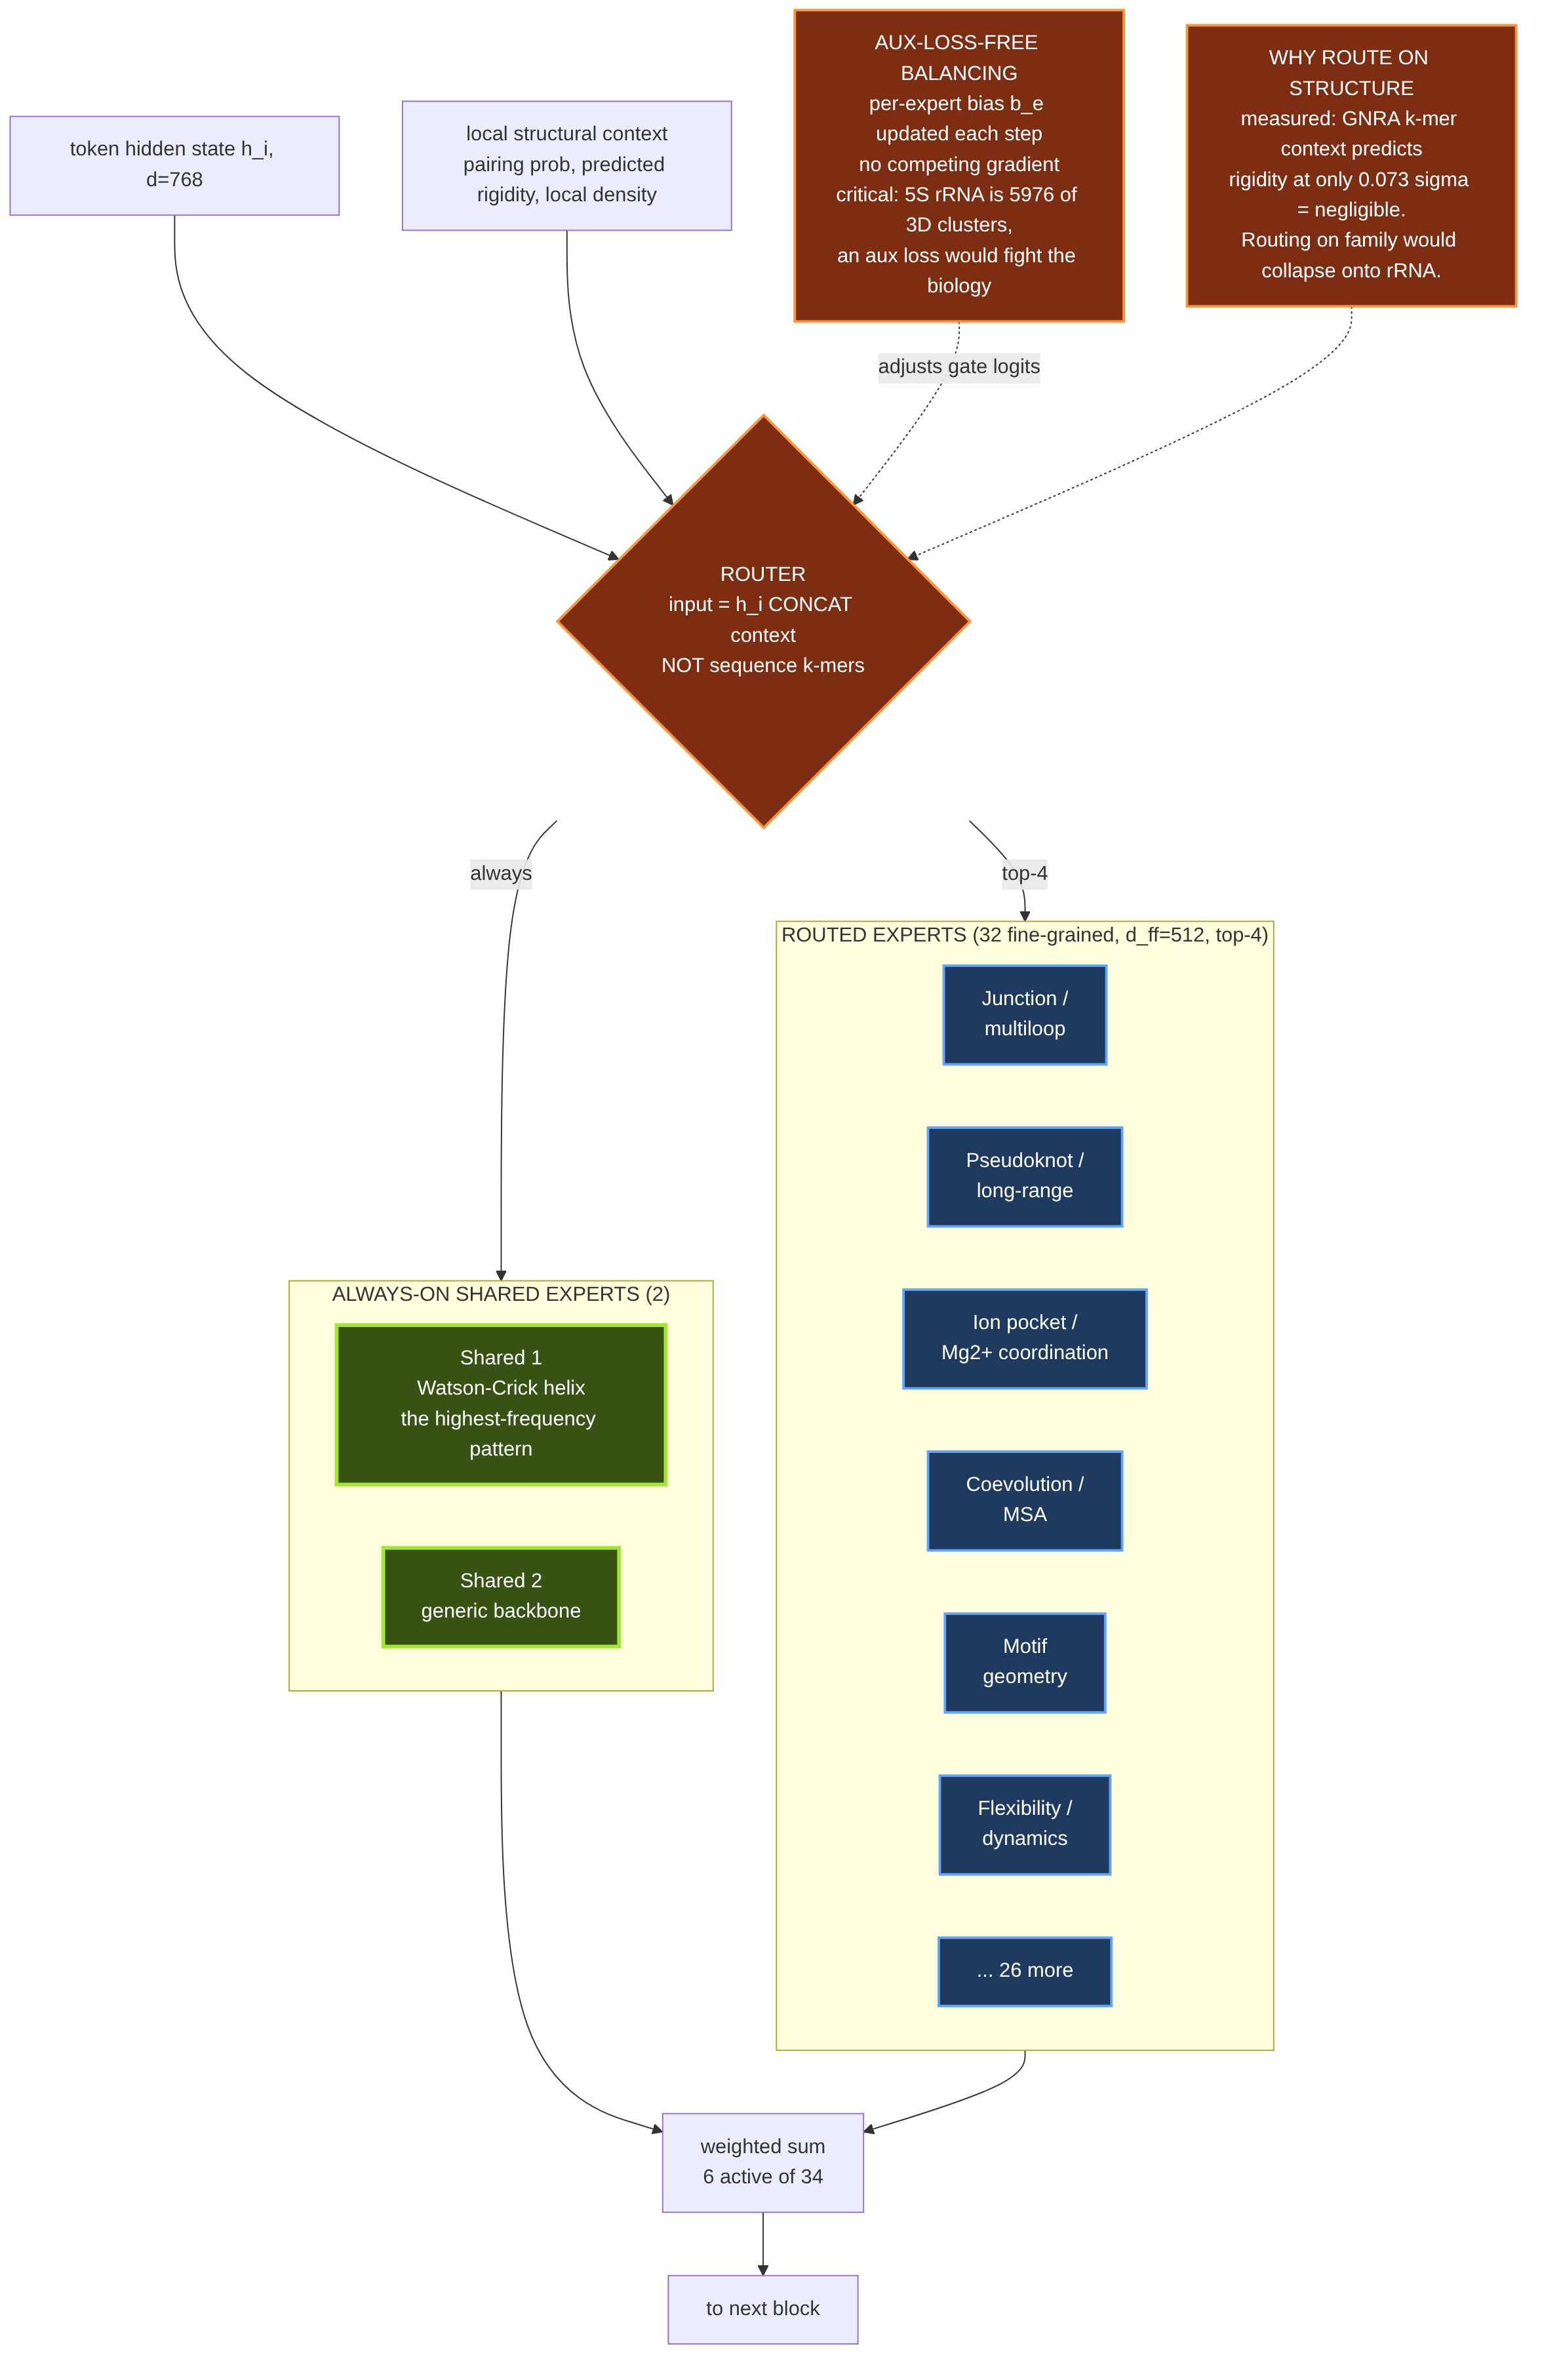
\includegraphics[height=0.78\textheight,keepaspectratio]{../architecture/diagrams/rendered/03-moe-routing.png}
\caption{Expert routing. Routing keys on local structural regime, not sequence.}
\end{figure}

Following DeepSeekMoE, the design uses 32 fine-grained routed experts at
$d_{\text{ff}} = 512$ plus 2 always-on shared experts, with top-4 routing giving
6 active experts of 34, in every second block.

Shared-expert isolation matters for a specific reason here: Watson--Crick helix
formation is the highest-frequency pattern in all RNA. Placing it in an
always-on shared expert prevents all 32 routed experts from separately
relearning it, freeing them to specialise on what is rare and hard---junctions,
pseudoknots and ion pockets.

Load balancing is auxiliary-loss-free, adjusting a per-expert bias each step
rather than adding a loss term. This matters acutely here because our 3D data is
pathologically imbalanced: 5S rRNA alone accounts for $5{,}976$ BGSU clusters,
so an auxiliary balance loss would actively fight the biology.

The router input is the token hidden state concatenated with the current local
structural estimate---pairing probability, predicted rigidity, local density---and
the alignment depth $N_{\text{eff}}/L$, which gates the coevolution expert
(Section~\ref{sec:coev}). This follows directly from the GNRA negative result of
Table~\ref{tab:gnra}: routing on sequence $k$-mers does not work. It also prevents router collapse
onto rRNA, because structural regimes are far more evenly distributed across the
corpus than families are.

\subsubsection{Parameter budget}

\begin{table}[h]
\centering
\caption{PHAROS-Base parameter budget against NucleicBERT.}
\label{tab:params}
\begin{tabular}{lrr}
\toprule
\textbf{Component} & \textbf{Total} & \textbf{Active} \\
\midrule
Embeddings (vocab 5)                 & 0.01M & 0.01M \\
Attention, 32 blocks, $d=768$        & 75.5M & 75.5M \\
MoE FFN, 16 blocks $\times$ 34 experts & 642M  & 113M \\
Dense FFN, 16 non-MoE blocks         & 113M  & 113M \\
Sparse pair track and triangle updates & 45M  & 45M \\
Motif bank, heads, decoder           & 35M   & 35M \\
\midrule
\textbf{PHAROS-Base total}           & $\mathbf{\sim 911M}$ & $\mathbf{\sim 382M}$ \\
NucleicBERT (dense)                  & 404M & 404M \\
\bottomrule
\end{tabular}
\end{table}

PHAROS-Base carries $2.3\times$ the capacity of NucleicBERT at slightly lower
active compute, with an attention term roughly $8\times$ cheaper at long context.

\subsection{Hierarchical pair track}
\label{sec:hpt}

\begin{figure}[p]
\centering
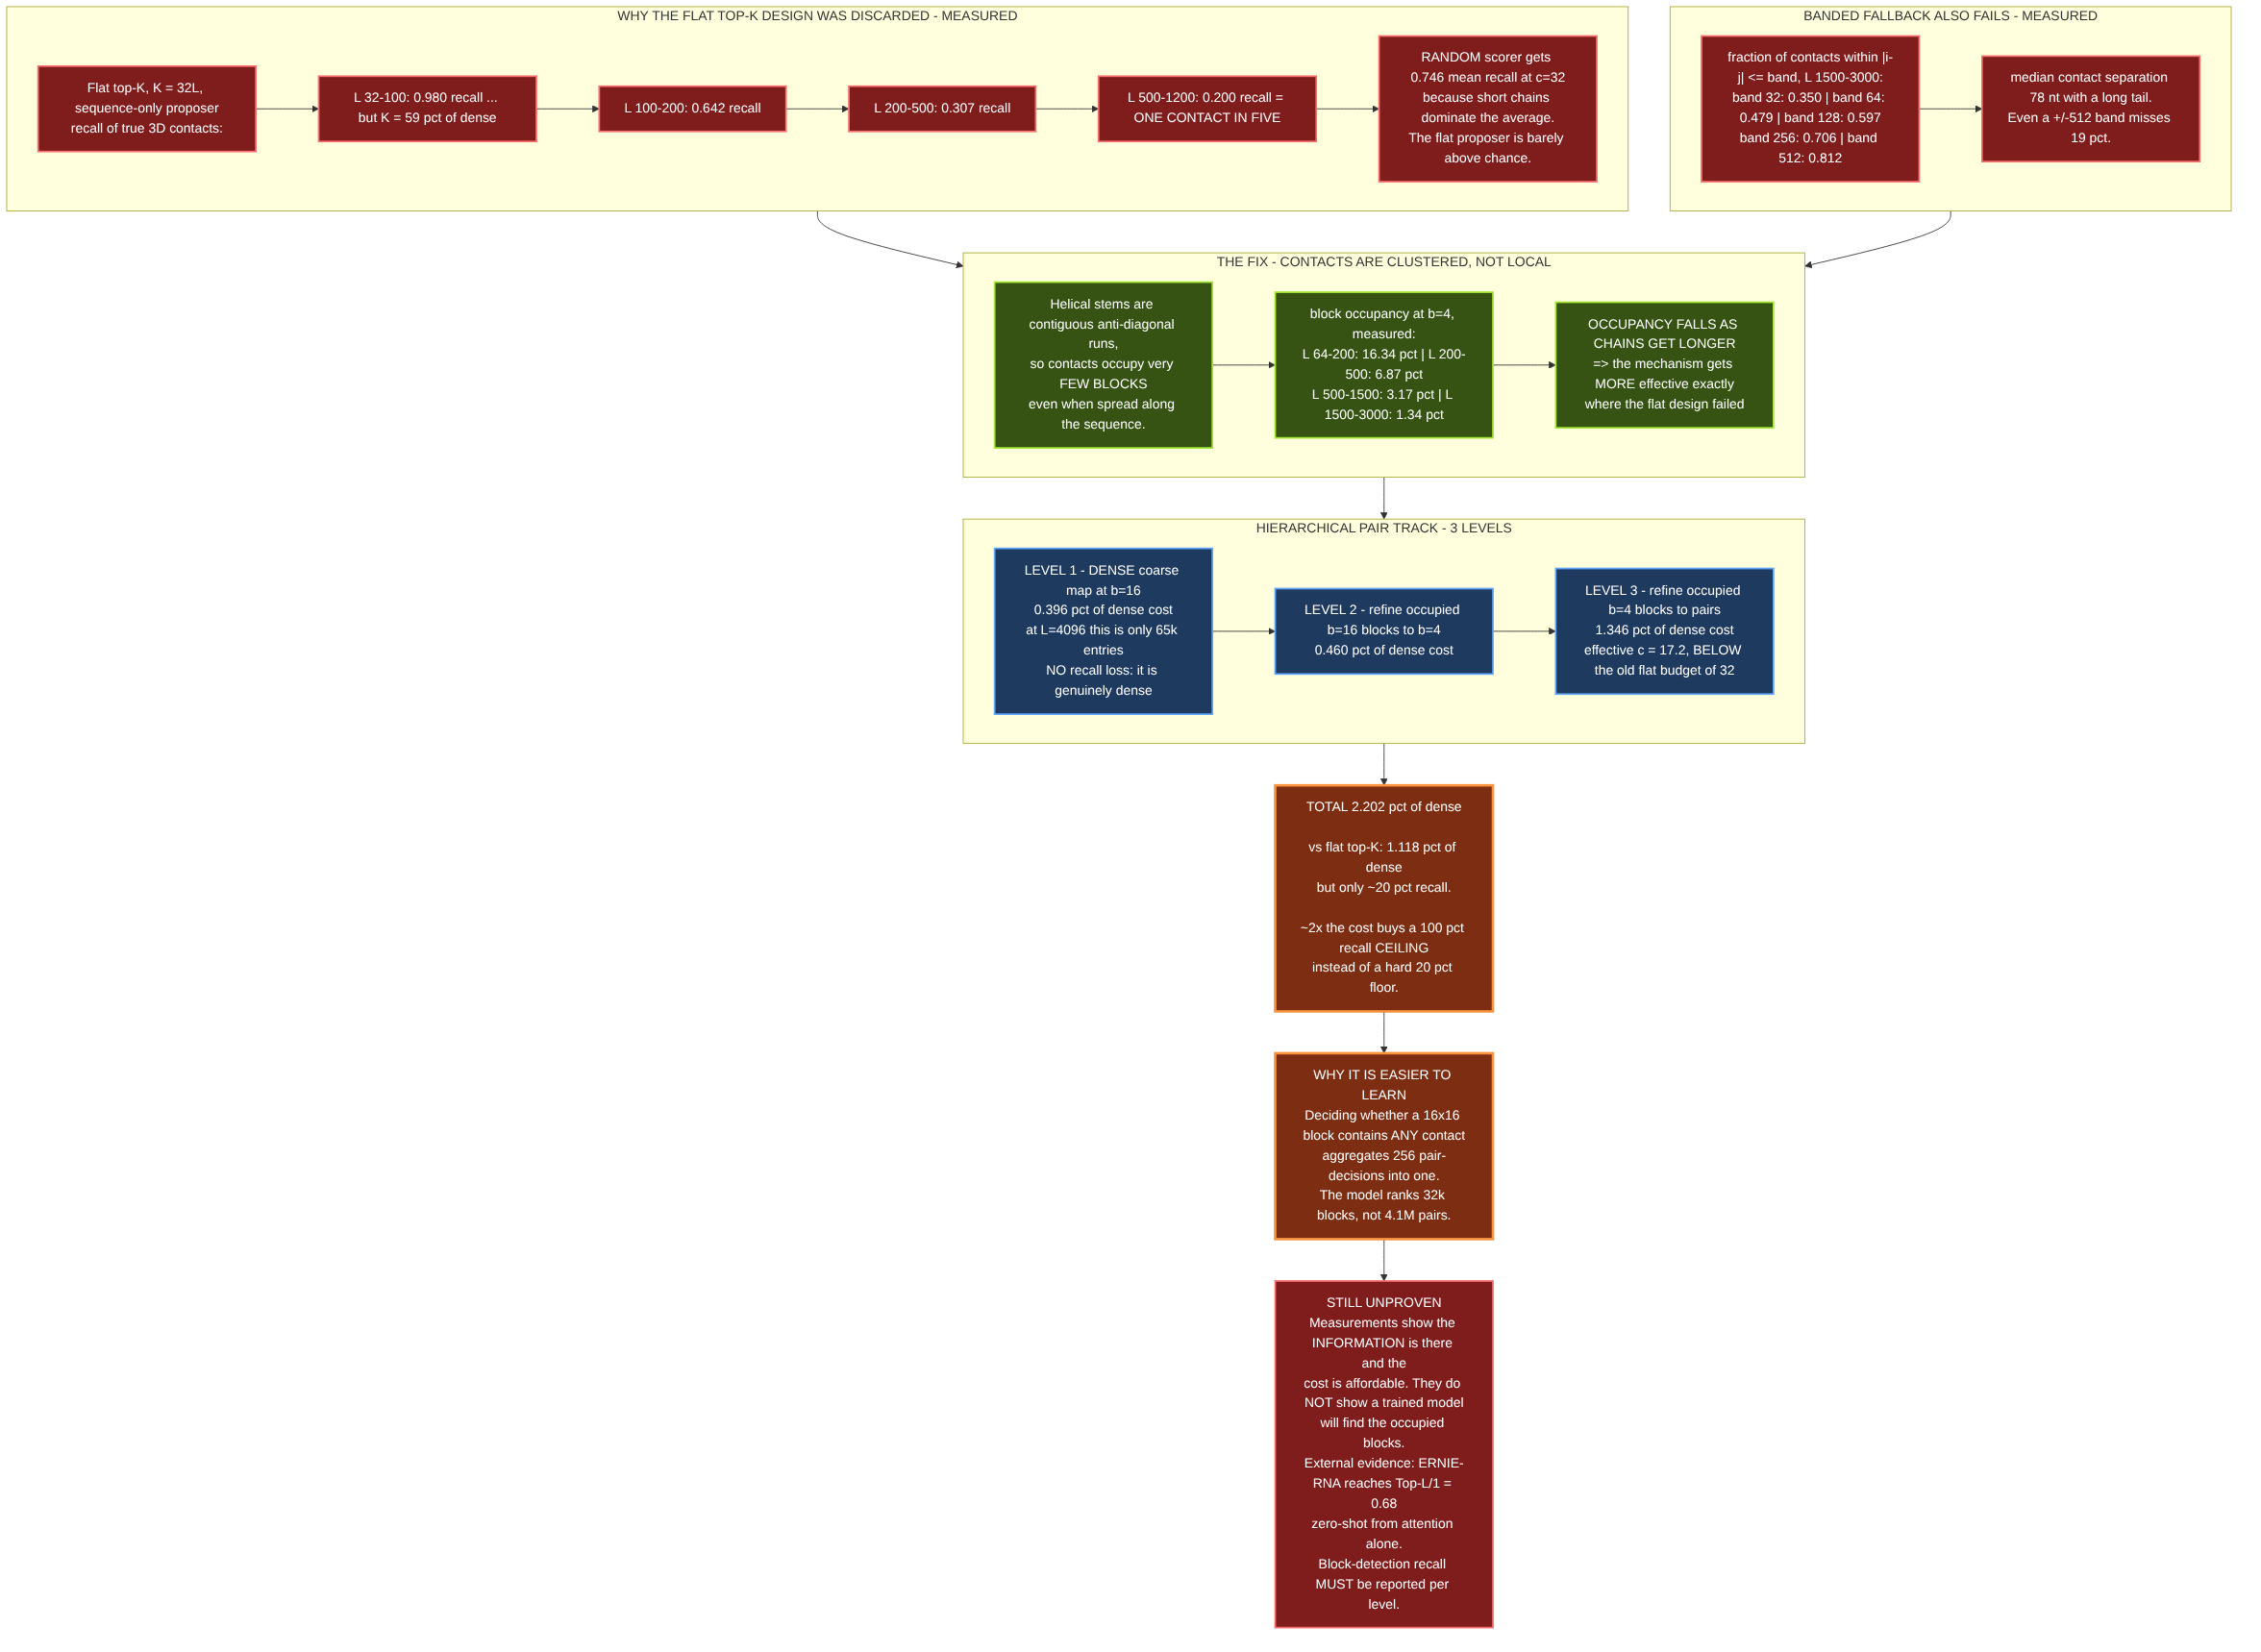
\includegraphics[width=\textwidth,keepaspectratio]{../architecture/diagrams/rendered/04-hierarchical-pair-track.png}
\caption{The pair track, after the flat design was measured and replaced.}
\end{figure}

\subsubsection{A flat top-$K$ proposal was specified, measured, and discarded}

Version 0.1 of this design specified a flat proposal retaining $K = 32L$
candidate edges. We tested it. Scoring every pair with a sequence-only proposer
(the ERNIE-RNA pair prior, stacking context, and an exponential
sequence-distance decay) and measuring recall of true 3D contacts within the top
$K$ gives Table~\ref{tab:recall}.

\begin{table}[h]
\centering
\caption{Recall of true 3D contacts under a flat top-$K$ proposal at $c=32$. \meas}
\label{tab:recall}
\begin{tabular}{lccc}
\toprule
\textbf{Chain length} & \textbf{$n$} & \textbf{mean recall} & \textbf{$K$ as \% of dense} \\
\midrule
32--100   & 29 & $0.980$ & $59.4\%$ \\
100--200  & 6  & $0.642$ & $25.5\%$ \\
200--500  & 3  & $0.307$ & $9.0\%$ \\
500--1200 & 5  & $\mathbf{0.200}$ & $4.7\%$ \\
\bottomrule
\end{tabular}
\end{table}

A \emph{random} scorer achieves mean recall $0.746$ at $c=32$ over the same
chains, because on short chains $32L$ already covers most of the map. The flat
proposer's headline mean of $0.795$ is therefore very nearly an artefact of
short chains. \textcolor{risk}{\textbf{On long chains, where sparsity actually
matters, it recovers one contact in five}}---a silent and fatal accuracy
ceiling.

A banded fallback does not rescue it, because RNA contacts are not sufficiently
local. The fraction of contacts within $|i-j| \leq$ band is $0.350$ at band 32,
$0.479$ at 64, $0.597$ at 128, $0.706$ at 256 and $0.812$ at 512 for chains of
1500--3000~nt; median contact separation is $78$~nt with a long tail. Even a
$\pm512$ band, which would cost vastly more than the whole budget, misses $19\%$.

\subsubsection{Contacts are clustered, so select blocks rather than pairs}

Helical stems are contiguous anti-diagonal runs in the contact map. Contacts are
therefore spread along the sequence but concentrated in very few
\emph{blocks}. Table~\ref{tab:blocks} measures this.

\begin{table}[h]
\centering
\caption{Block occupancy at block size $b=4$: the fraction of blocks containing
at least one contact, and the effective $c$ of keeping every occupied block. \meas}
\label{tab:blocks}
\begin{tabular}{lccc}
\toprule
\textbf{Chain length} & \textbf{median $L$} & \textbf{occupancy at $b=4$} & \textbf{effective $c$} \\
\midrule
64--200    & 88   & $16.34\%$ & $7.9$ \\
200--500   & 393  & $6.87\%$  & $12.6$ \\
500--1500  & 1038 & $3.17\%$  & $14.8$ \\
1500--3000 & 2861 & $\mathbf{1.34\%}$ & $\mathbf{17.2}$ \\
\bottomrule
\end{tabular}
\end{table}

Occupancy \emph{falls} as chains lengthen, so the mechanism becomes more
effective at exactly the lengths where the flat design failed. Retaining every
occupied $4\times4$ block costs an effective $c$ of roughly $17$---below the
discarded flat budget of $32$---while capturing every contact by construction.

\subsubsection{Three-level coarse-to-fine track}

\begin{table}[h]
\centering
\caption{Cost of the hierarchical track at $L = 2861$, as a fraction of a dense
pair map. \meas}
\begin{tabular}{llc}
\toprule
\textbf{Level} & \textbf{Operation} & \textbf{Cost} \\
\midrule
L1 & \textbf{dense} pair map at block size $b=16$ & $0.396\%$ \\
L2 & refine occupied $b=16$ blocks to $b=4$ & $0.460\%$ \\
L3 & refine occupied $b=4$ blocks to individual pairs & $1.346\%$ \\
\midrule
& \textbf{Total} & $\mathbf{2.202\%}$ \\
& flat top-$K$ at $c=32$, for comparison & $1.118\%$ (at $\sim$20\% recall) \\
\bottomrule
\end{tabular}
\end{table}

For roughly twice the cost of the flat design, the track moves from a hard
$20\%$ recall ceiling to a ceiling of $100\%$. Two properties make this work.
First, the L1 map is \emph{genuinely dense}, so it loses no recall at the coarse
level at all---at $L=4096$ with $b=16$ it is only $65$k entries. Recall can only
be lost at the selection thresholds, which are tunable and can be set
recall-first. Second, deciding whether a $16\times16$ block contains any contact
aggregates $256$ pair-decisions into one, so coarse-level signal-to-noise is far
higher than for individual pair ranking. The model ranks $32$k blocks and then
$16$ sub-blocks inside each survivor, never $4.1$M individual pairs.

\subsubsection{Reference implementation and measured cost}

The cost arithmetic above is turned into running code in
\texttt{research/architecture/reference/}, and measured against an
AlphaFold3-style dense baseline on the machine this report was prepared on
(CPU only, 14~GB RAM, no CUDA), at batch 1, $d_{\text{model}}=768$,
$d_{\text{pair}}=128$, $b_1=16$, $b_2=4$ and budget $c=20$.

\begin{table}[h]
\centering
\caption{Hierarchical track versus dense baseline, measured. \meas}
\label{tab:bench}
\small
\begin{tabular}{rrrrrrr}
\toprule
\textbf{$L$} & \textbf{HPT time} & \textbf{HPT pairs} & \textbf{\% of dense} & \textbf{eff.\ $c$} & \textbf{Dense time} & \textbf{Dense peak RSS} \\
\midrule
128  & 0.01 s & 750    & $9.23\%$  & 5.9  & 0.07 s & 0.10 GB \\
256  & 0.01 s & 3{,}506  & $10.74\%$ & 13.7 & 0.28 s & 0.33 GB \\
512  & 0.05 s & 10{,}054 & $7.69\%$  & 19.6 & 1.22 s & 1.30 GB \\
1024 & $\mathbf{0.10}$ s & 20{,}102 & $3.84\%$ & 19.6 & $\mathbf{8.26}$ s & $\mathbf{5.15}$ GB \\
2048 & 0.33 s & 40{,}198 & $1.92\%$  & 19.6 & \emph{not runnable} & predicted 12.9 GB \\
4096 & $\mathbf{0.45}$ s & 80{,}390 & $\mathbf{0.96\%}$ & 19.6 & \emph{not runnable} & predicted 51.5 GB \\
\bottomrule
\end{tabular}
\end{table}

Two things are established that arithmetic alone could not. First, the dense
baseline genuinely does not run: it needs a predicted 12.9~GB of activations at
$L=2048$ and 51.5~GB at $L=4096$ on a 14~GB machine, so the infeasibility claim
is not rhetorical. Second, at the largest length both can run, the hierarchical
track is roughly $83\times$ faster (0.10~s versus 8.26~s) with peak resident
memory below measurement noise against the baseline's 5.15~GB.

The cost fraction falls monotonically with length, from $9.2\%$ to $0.96\%$,
because the budget grows as $cL$ while the dense map grows as $L^2$. The
mechanism becomes cheaper relative to dense exactly where it is needed,
mirroring the falling block occupancy of Table~\ref{tab:blocks}.

\paragraph{Two silent defects found while building it.} Both would have degraded
a trained model rather than crashing. The L3 expansion initially paired block
rows with block columns element-wise, materialising only each block's
\emph{diagonal}---4 pairs per $4\times4$ block instead of 16---silently
delivering a quarter of the intended budget. Separately, the L2 selection budget
was expressed as a fraction of all pairs and was clamped by masking to a quarter
of its target. Both pinned the effective $c$ at $5.0$ while the code appeared to
work. Budgets are now stated in the same units as the measurement ($K = cL$
pairs) so any mismatch is immediately visible.

\paragraph{What remains unproven.} These measurements establish that the
information is present and the cost affordable. They do \emph{not} establish
that a trained model will identify occupied blocks accurately; that requires
training. The relevant external evidence is ERNIE-RNA's zero-shot Top-$L$/1
contact precision of $0.68$ from attention maps alone, which indicates that
learned representations rank contacts far better than the sequence-only
heuristic tested above. \textcolor{risk}{\textbf{Block-detection recall must be
reported per length bin and per level.}}

\subsection{Motif retrieval bank}

The RNA 3D Motif Atlas 4.12 compresses $4{,}992$ loop instances into $667$ motif
classes, $413$ internal and $254$ hairpin: a $7.5\!:\!1$ ratio indicating that
RNA tertiary structure is far more repetitive than its sequence diversity
suggests. PHAROS precomputes a frozen key--value bank over these classes, with
keys encoding the non-canonical interaction-graph signature and values encoding
internal geometry as distance-matrix eigenfeatures plus a backbone torsion
profile. The pair track cross-attends into this bank.

This is the appropriate response to data scarcity. With only $6{,}661$ unique
sequences carrying 3D structure, a model cannot reliably learn motif geometry
implicitly. The bank supplies the geometry explicitly, leaving the model to
learn only \emph{where} motifs occur---a substantially easier problem than
learning what they look like. The bank is roughly $10^3$ fixed entries shared
across a batch, so its cost is negligible. Consistent with
Table~\ref{tab:gnra}, retrieval is keyed on the interaction graph, never on
sequence $k$-mers.

\subsection{Physics module}

\begin{figure}[h]
\centering
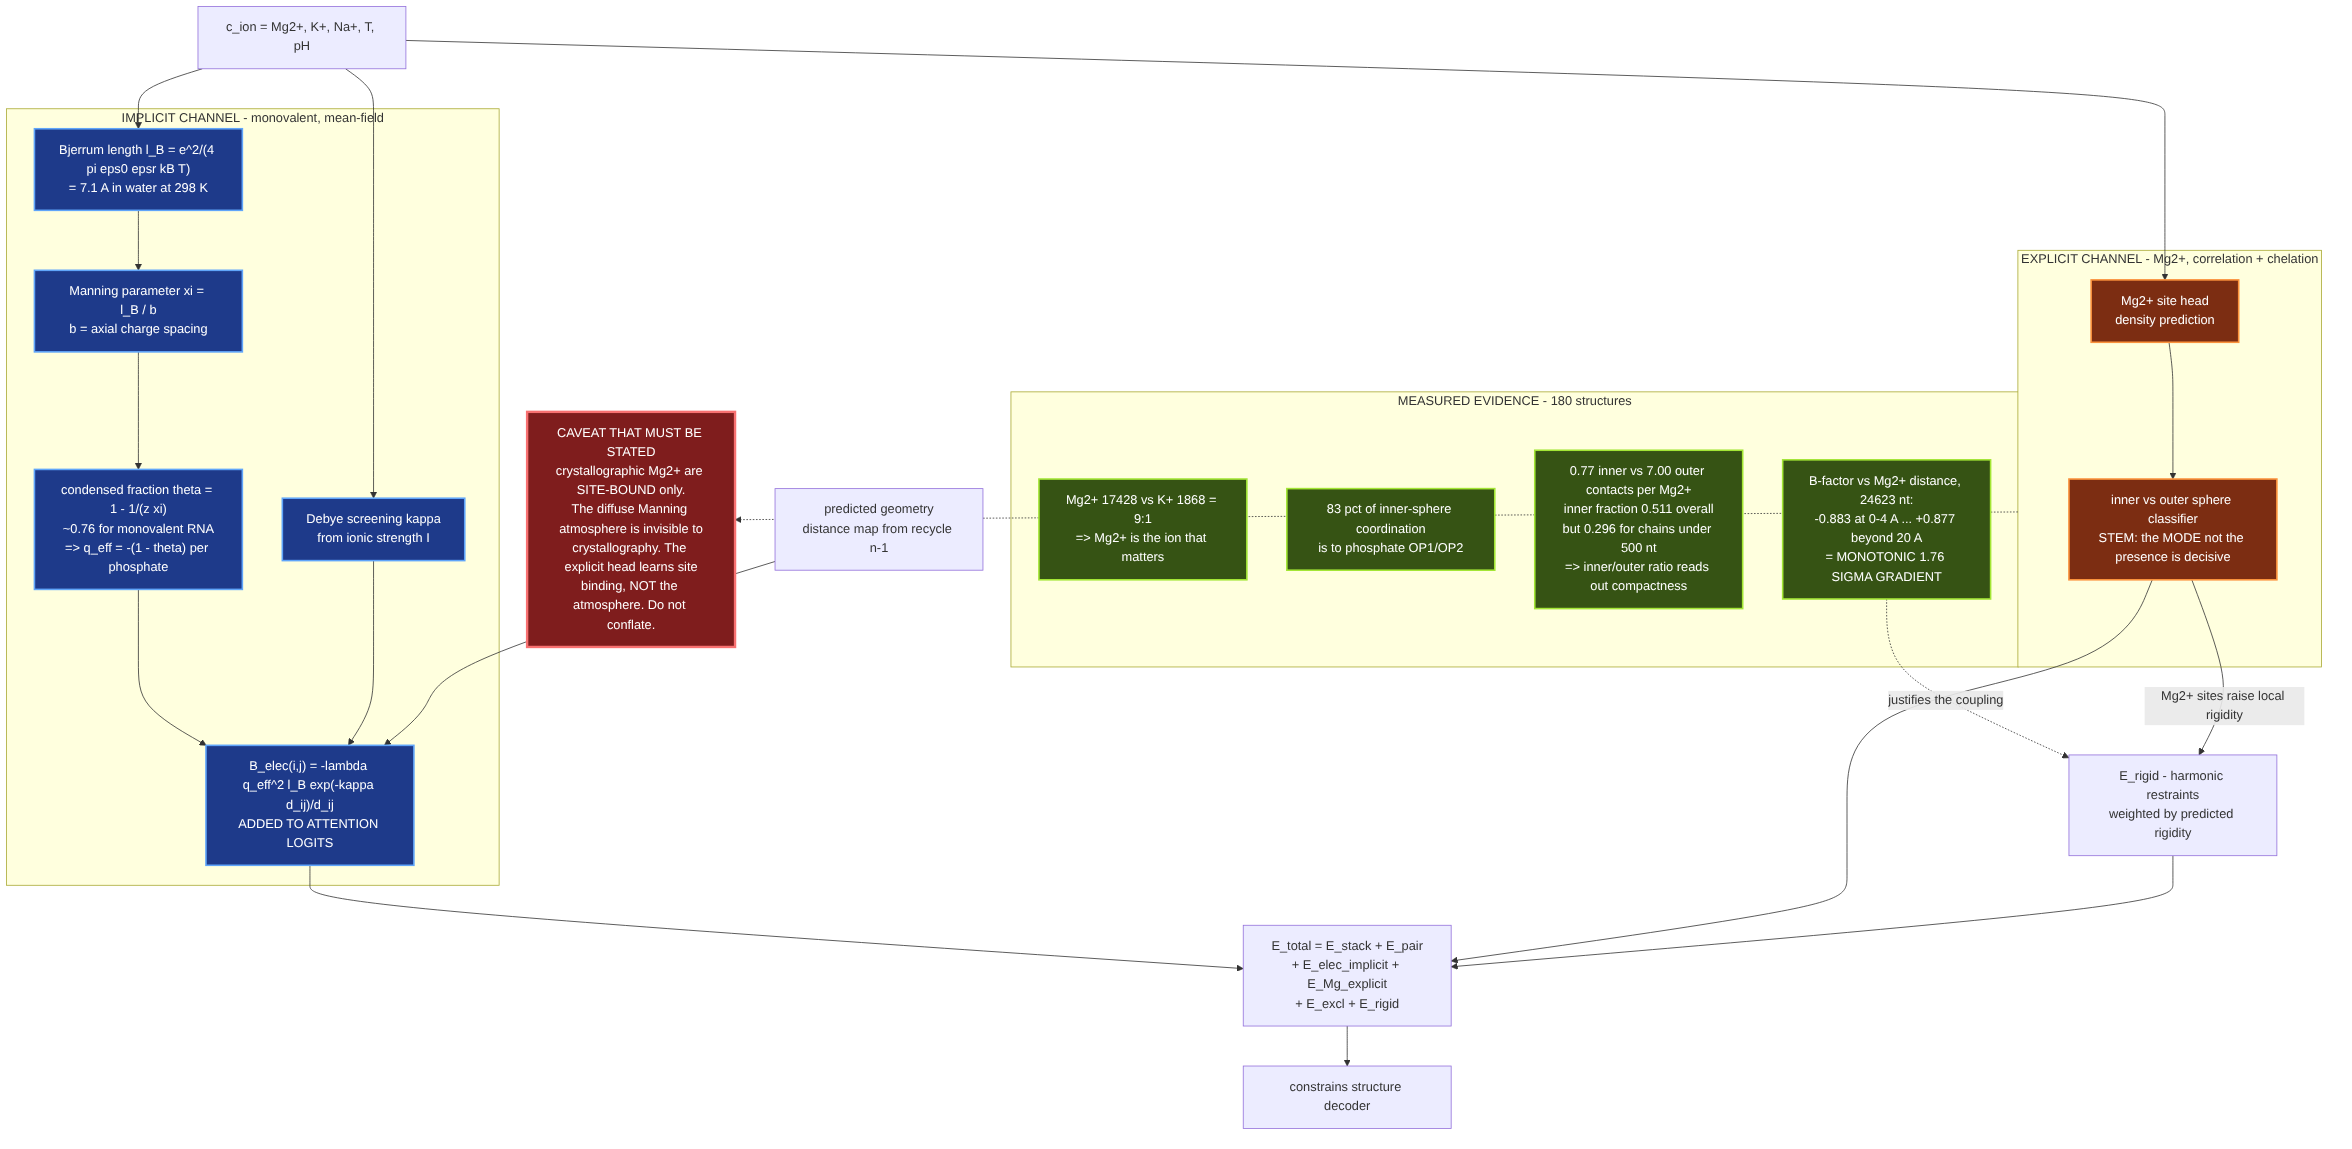
\includegraphics[width=\textwidth,keepaspectratio]{../architecture/diagrams/rendered/05-physics-hamiltonian.png}
\caption{The hybrid implicit/explicit electrostatic treatment.}
\end{figure}

A differentiable energy is evaluated on the predicted geometry:
\begin{equation}
E_{\text{total}} = E_{\text{stack}} + E_{\text{pair}}
+ E_{\text{elec}}^{\text{implicit}} + E_{\mathrm{Mg}}^{\text{explicit}}
+ E_{\text{excl}} + E_{\text{rigid}}.
\end{equation}

The implicit/explicit split follows STEM, which establishes that mean-field
theory captures monovalent KCl well but fails for $\mathrm{Mg}^{2+}$, where
ion--ion correlation and site-specific chelation dominate. Our own inventory
agrees on which species matters: $\mathrm{Mg}^{2+}$ outnumbers $\mathrm{K}^{+}$
by $9\!:\!1$.

Inner/outer-sphere classification is a first-class output because STEM's central
claim is that folding dynamics are driven by \emph{exchange between} direct and
water-mediated coordination---the mode, not the presence, is decisive. Our
measurements supply both channels directly and show the inner fraction varies
with compactness ($0.511$ overall, $0.296$ below $500$~nt).

The term $E_{\text{rigid}}$ closes the loop with Table~\ref{tab:mgrigid}:
predicted $\mathrm{Mg}^{2+}$ sites raise local rigidity, which stiffens harmonic
restraints, which constrains the decoder. That pathway is the architectural
encoding of the measured $1.76\sigma$ gradient.

\subsection{Heads and decoder}

\begin{table}[h]
\centering
\caption{Prediction heads and their supervision. Two channels are effectively free.}
\label{tab:heads}
\small
\begin{tabular}{@{}llll@{}}
\toprule
\textbf{Head} & \textbf{Supervision source} & \textbf{Status} & \textbf{Labels} \\
\midrule
Secondary structure & bpRNA, ArchiveII, RNAStrAlign & in catalogue & $\sim$160k \\
Contact / distance  & RNA3DB, gRNAde & in catalogue & 27{,}452 chains \\
$\mathrm{Mg}^{2+}$ sites & \textbf{extracted from mmCIF} & \textbf{free} & 17{,}428 (180 structs) \\
Rigidity ($z_B$, RMSF) & \textbf{B-factors in mmCIF} & \textbf{free} & every X-ray struct \\
Reactivity (SHAPE/DMS) & Ribonanza / RMDB & \textbf{not acquired} & --- \\
3D coordinates & RNA3DB & in catalogue & 6{,}661 unique seqs \\
\bottomrule
\end{tabular}
\end{table}

The decoder is frame-based diffusion. We retain an explicit geometric and
energetic stage rather than going fully generative, consistent with the CASP16
observation that physics-plus-ML hybrids currently lead in RNA and with
trRosettaRNA's restraint-then-fold approach outscoring AlphaFold3's raw-atom
diffusion.

$\mathrm{Mg}^{2+}$ sites and B-factor rigidity deserve emphasis: both are
already present inside every mmCIF file the field routinely downloads, are used
by no current structure predictor, and were extracted end-to-end in preparing
this report.

%========================================================
\section{Ionic-condition supervision: an audit that rescoped the claim}
\label{sec:r2}

The headline novelty is accepting ionic conditions as an input. That requires
structures labelled with the ionic environment they were solved in, so we
audited all 180 sampled structures. The result changed the claim.

\subsection{Coverage is roughly one third, split across two storage conventions}

\begin{table}[h]
\centering
\caption{Where ionic conditions live, and how often they are populated. \meas}
\begin{tabular}{lclc}
\toprule
\textbf{Method} & \textbf{$n$} & \textbf{mmCIF location} & \textbf{usable ionic vector} \\
\midrule
Cryo-EM & 117 & \texttt{\_em\_buffer\_component} (structured) & $\mathbf{23.9\%}$ \\
X-ray   & 63  & \texttt{\_exptl\_crystal\_grow.pdbx\_details} (free text) & $58.7\%$ mention an ion \\
\bottomrule
\end{tabular}
\end{table}

Cryo-EM entries record pH for $94\%$ of structures but populate
\texttt{\_em\_buffer\_component} for only $24.8\%$. X-ray entries always carry
crystallisation details, but as prose---``0.1--0.2 M Arginine-HCl, 0.1M Tris-HCl
pH 7.6, 2.6--3.0\% PEG-20K''---so extraction is noisy. Combined, about $36\%$ of
structures yield any recoverable ionic condition: trainable, but a threefold
reduction in usable 3D data for that stage.

\subsection{The deeper problem: the PDB is survivorship-biased on ionic conditions}

Where Mg\textsuperscript{2+} concentration \emph{is} recorded, its range is narrow.

\begin{table}[h]
\centering
\caption{Recorded buffer concentrations in cryo-EM entries. \meas}
\begin{tabular}{lcccc}
\toprule
\textbf{Ion} & \textbf{$n$} & \textbf{p10} & \textbf{median} & \textbf{p90} \\
\midrule
Mg\textsuperscript{2+} & 21 & 5.0 mM & $\mathbf{7.5}$ mM & 15.0 mM \\
K\textsuperscript{+}   & 13 & 30 mM  & 100 mM & 150 mM \\
Na\textsuperscript{+}  & 12 & 100 mM & 150 mM & 150 mM \\
\bottomrule
\end{tabular}
\end{table}

Mg\textsuperscript{2+} spans only 5--15 mM. This is not a sampling accident:
\textbf{nobody deposits a structure of unfolded RNA}. Every PDB entry was solved
under conditions chosen \emph{because} the RNA folds there, so the archive
contains almost no contrast between folding and non-folding ionic regimes.

\begin{quote}
\textcolor{risk}{\textbf{Consequence.}} The $[\mathrm{Mg}^{2+}] \rightarrow$
structure response cannot be learned from the PDB. A model trained only on
deposited structures would observe ionic condition as a near-constant and would
correctly learn to ignore it.
\end{quote}

\subsection{How the claim is rescoped}

The novelty splits into three components with very different evidentiary support.

\begin{table}[h]
\centering
\begin{tabular}{>{\raggedright\arraybackslash}p{5.2cm}>{\raggedright\arraybackslash}p{5.6cm}>{\raggedright\arraybackslash}p{3.4cm}}
\toprule
\textbf{Component} & \textbf{Support} & \textbf{Status} \\
\midrule
$B_{\mathrm{elec}}$ Manning/Debye screening & closed-form physics; needs no training labels & \textbf{unaffected} \\
Mg\textsuperscript{2+} site head and inner/outer classifier & 17{,}428 labelled ions from 180 structures & \textbf{well supported} \\
Learned \emph{response} to varying ionic conditions & requires titration series; the PDB has none & \textcolor{risk}{\textbf{not supported}} \\
\bottomrule
\end{tabular}
\end{table}

The first two stand unchanged. The third must be dropped or supplied from data
the PDB cannot provide: \textbf{RMDB Mg\textsuperscript{2+} titration series}
(SHAPE/DMS probing across an Mg\textsuperscript{2+} ladder on the same sequence)
and SAXS Mg\textsuperscript{2+} titrations measuring compaction. Training stage 5
as originally specified---ion-conditioned refinement on structures stratified by
ionic condition---\textbf{is not viable on PDB data alone} and is rewritten to
condition on probing titrations, with deposited structures supplying only
site-level supervision.

This promotes chemical-probing acquisition from ``most valuable missing asset''
to \textbf{prerequisite for the headline claim}. Note that Ribonanza alone does
not supply it; the Mg\textsuperscript{2+} titration series in RMDB do.

\section{Data mapping and the acquisition gap}
\label{sec:gap}

\begin{figure}[p]
\centering
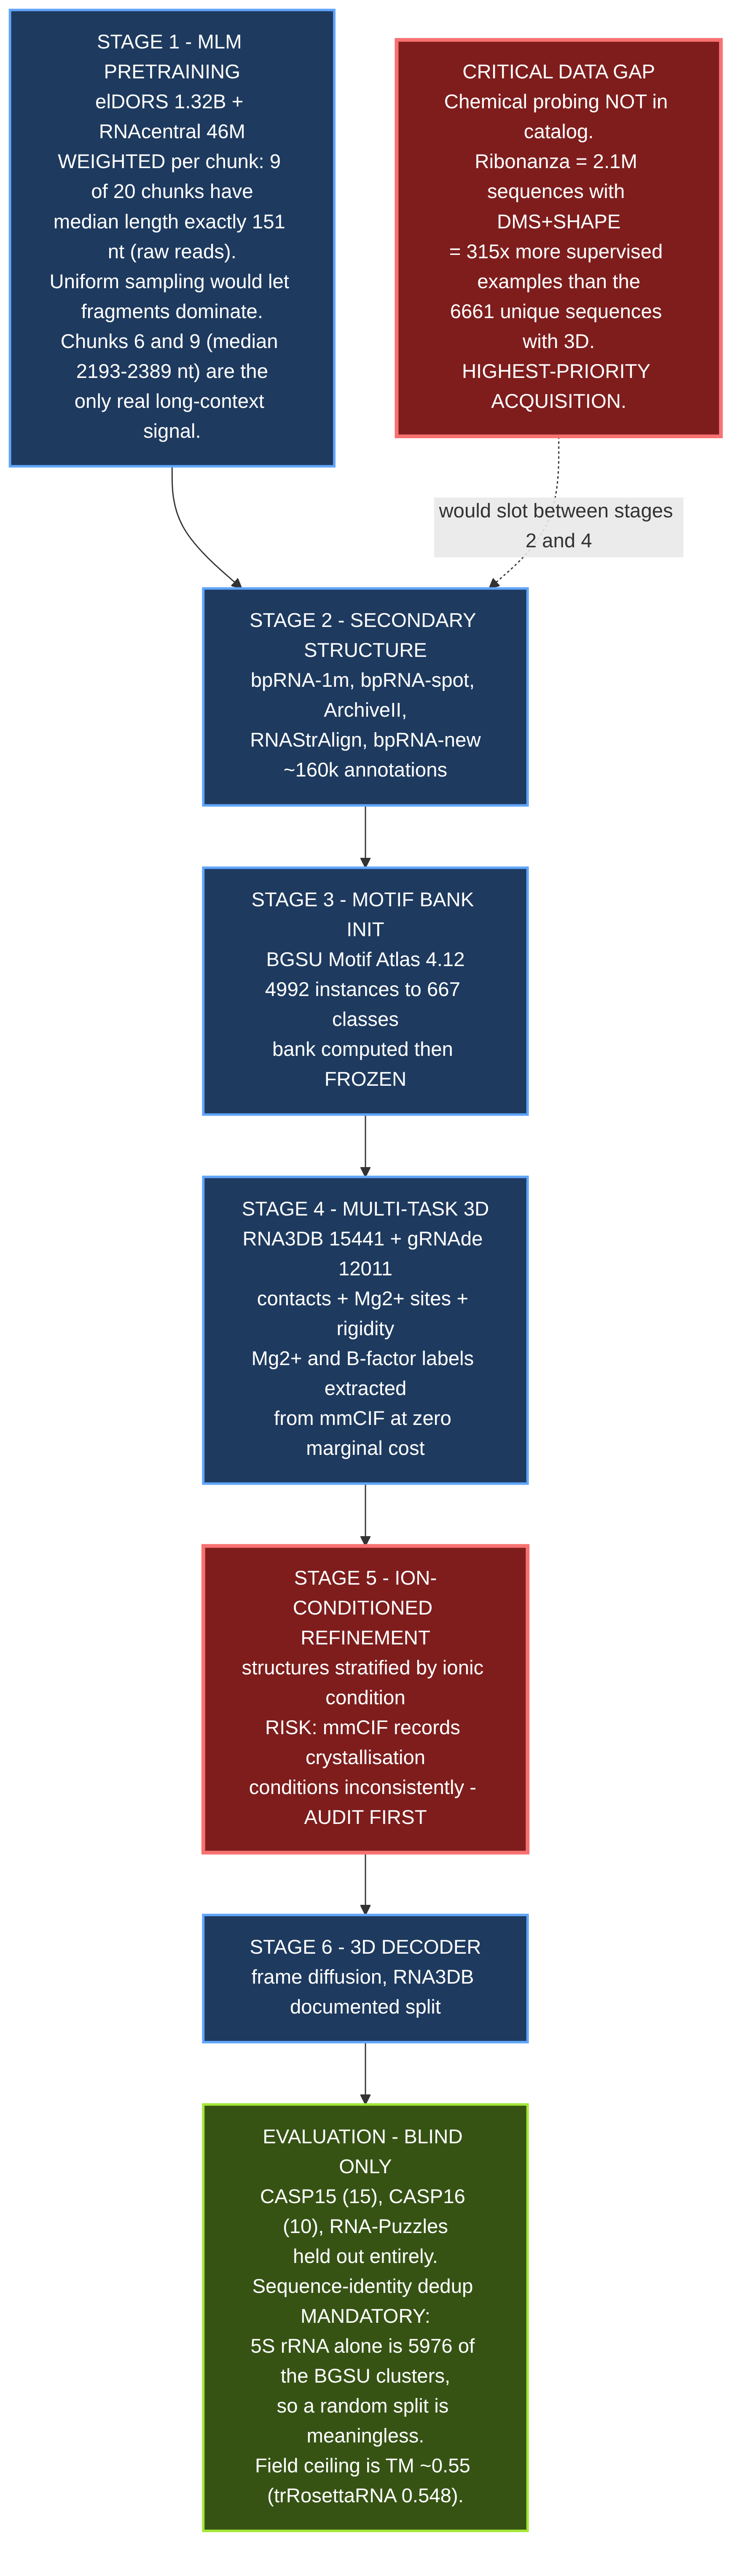
\includegraphics[height=0.82\textheight,keepaspectratio]{../architecture/diagrams/rendered/06-training-curriculum.png}
\caption{Training curriculum, data sources, and the chemical-probing gap.}
\end{figure}

Six of seven training stages are fully served by the existing catalogue. The
exception is chemical probing, and it is the most valuable missing asset.
Ribonanza provides $2.1$M sequences with DMS and SHAPE measurements---roughly
$315\times$ more supervised examples than the $6{,}661$ unique sequences with 3D
structure. It is the only label source that is simultaneously abundant,
structure-informative and already public. This is the highest-priority
acquisition.

\paragraph{Corpus weighting.} The elDORS chunks are source-partitioned rather
than homogeneous: 9 of 20 chunks have a median length of exactly $151$~nt,
indicating unassembled sequencing reads, while chunks 6 and 9 (median
$2{,}193$--$2{,}389$~nt) are the only substantial source of long-context signal.
Uniform sampling in Stage 1 would allow read fragments to dominate pretraining,
so per-chunk weighting is required.

%========================================================
\section{Novelty claims}

\begin{table}[h]
\centering
\caption{Novelty claims stated precisely, with prior-art status.}
\begin{tabular}{p{6.6cm}p{8.2cm}}
\toprule
\textbf{Claim} & \textbf{Prior-art status} \\
\midrule
Ionic conditions as a model input, reaching attention logits through a
Manning-screened Coulomb bias & No existing RNA structure predictor accepts
ionic conditions. The physics term needs no labels; the learned response
requires titration data (Section~\ref{sec:r2}). \\
First sparse-MoE architecture for RNA structure & AIDO.Protein is MoE for
protein; no RNA equivalent exists. \\
Hierarchical coarse-to-fine pair track selecting blocks rather than pairs,
justified by measured $1.34\%$ block occupancy & AlphaFold3 and Rhoformer are
dense $O(L^2)$; flat top-$K$ sparsification is measured here to fail at
$\sim$20\% recall on long chains. \\
Frozen motif KV bank as a retrieval-based geometry prior & The Motif Atlas is
published but wired into no large model. \\
$\mathrm{Mg}^{2+}$ sites and B-factor rigidity as free auxiliary supervision &
Present in mmCIF; used by no structure predictor. \\
Coupled ion--rigidity expert justified by a measured $1.76\sigma$ gradient &
Treated separately or not at all elsewhere. \\
\bottomrule
\end{tabular}
\end{table}

%========================================================
\section{Risks and open questions}

\begin{enumerate}[leftmargin=1.4em,itemsep=0.25em]
\item \textbf{Block-detection recall.} Superseded but not eliminated. The flat
top-$K$ design was measured at $\sim$20\% recall on long chains and replaced
(Section~\ref{sec:hpt}). The hierarchical track has a $100\%$ recall
\emph{ceiling} by construction, but whether a trained model attains it is
unproven. Recall must be reported per length bin and per level.
\item \textbf{Ionic metadata sparsity---audited, partially confirmed}
(Section~\ref{sec:r2}). About $36\%$ of structures yield a recoverable ionic
condition. Worse, recorded Mg\textsuperscript{2+} spans only 5--15 mM because
the PDB is survivorship-biased. The learned ionic response must come from RMDB
titration series, not the PDB. The closed-form physics term and the
Mg\textsuperscript{2+} site head are unaffected.
\item \textbf{Crystallographic ions are not the solution ensemble.} The explicit
head learns site binding, not the diffuse atmosphere. These must not be
conflated.
\item \textbf{B-factor is a noisy rigidity proxy.} Excluding cryo-EM left only
31 of 137 parsed structures usable, which materially shrinks the rigidity label
set.
\item \textbf{Association, not isolated causation.} $\mathrm{Mg}^{2+}$ proximity
and packing density both track folded cores.
\item \textbf{Infrastructure.} NucleicBERT used 192 A100s densely. MoE improves
FLOP efficiency but adds routing and communication complexity.
\item \textbf{Evaluation honesty.} The field ceiling is TM $\approx 0.55$. Any
improvement claim must be made on blind sets---CASP15/16 and RNA-Puzzles---never
on rRNA-saturated random splits. Sequence-identity deduplication is mandatory.
\end{enumerate}

%========================================================
\section{Status}

This is a design specification. No model has been trained and no predictive
performance is claimed. What has been established is the evidentiary basis:
the contact-scaling law, the ion--rigidity coupling, the ion inventory and
coordination chemistry, and the GNRA negative result, all measured on 180
non-redundant structures with reproducible scripts. The next phase is to
implement the sparse pair track and validate proposal recall before any
large-scale training is attempted.

\appendix
\section{Reproducing the measurements}

\begin{table}[h]
\centering
\small
\begin{tabular}{@{}ll@{}}
\toprule
\textbf{Script} & \textbf{Output} \\
\midrule
\texttt{.../sampling/fetch\_samples.py} & 180 mmCIF, 12 Rfam seeds \\
\texttt{.../sampling/analyze\_ions\_motifs.py} & \texttt{ion\_summary.json} \\
\texttt{.../sampling/analyze\_rigidity.py} & \texttt{rigidity\_summary.json} \\
\texttt{.../sampling/analyze\_contact\_sparsity.py} & \texttt{contact\_sparsity.json} \\
\texttt{.../sampling/validate\_proposal\_recall.py} & \texttt{proposal\_recall.json} \\
\texttt{.../sampling/analyze\_contact\_separation.py} & \texttt{contact\_separation.json} \\
\texttt{.../sampling/analyze\_block\_sparsity.py} & \texttt{block\_sparsity.json} \\
\texttt{.../sampling/audit\_ionic\_metadata.py} & \texttt{ionic\_metadata\_audit.json} \\
\texttt{.../sampling/audit\_em\_buffers.py} & \texttt{em\_buffer\_audit.json} \\
\texttt{.../sampling/measure\_coevolution.py} & \texttt{coevolution\_signal.json} \\
\texttt{.../reference/benchmark\_pair\_track.py} & \texttt{pair\_track\_benchmark.json} \\
\bottomrule
\end{tabular}
\end{table}

\begin{thebibliography}{99}
\small
\bibitem{ernie} ERNIE-RNA: an RNA language model with structure-enhanced
representations. \emph{Nature Communications}, 2025.
\url{https://pmc.ncbi.nlm.nih.gov/articles/PMC12627772/}
\bibitem{rhofold} Accurate RNA 3D structure prediction using a language
model-based deep learning approach (RhoFold+). \emph{Nature Methods}, 2024.
\url{https://pmc.ncbi.nlm.nih.gov/articles/PMC11621015/}
\bibitem{af3} Accurate structure prediction of biomolecular interactions with
AlphaFold 3. \emph{Nature}, 2024.
\url{https://www.ncbi.nlm.nih.gov/pmc/articles/PMC11168924/}
\bibitem{stem} Structural Topology-based Electrostatic Model (STEM) Reveals
Ion-Coordination Exchange as a Driver of RNA Folding Dynamics, 2026.
\url{https://pmc.ncbi.nlm.nih.gov/articles/PMC13345221/}
\bibitem{manning} Generalized Manning Condensation Model Captures the RNA Ion
Atmosphere, 2015. \url{https://pubmed.ncbi.nlm.nih.gov/26197147/}
\bibitem{motif} The RNA 3D Motif Atlas: Computational methods for extraction,
organization and evaluation of RNA motifs. \emph{Methods}, 2016.
\url{https://pmc.ncbi.nlm.nih.gov/articles/PMC4921307/}
\bibitem{ribonanza} Ribonanza: deep learning of RNA structure through dual
crowdsourcing, 2024.
\url{https://www.ncbi.nlm.nih.gov/pmc/articles/PMC10925082/}
\bibitem{deepseekmoe} DeepSeekMoE: Towards Ultimate Expert Specialization in
Mixture-of-Experts Language Models, 2024.
\url{https://arxiv.org/html/2401.06066v1}
\bibitem{dsv3} DeepSeek-V3 Technical Report, 2024.
\url{https://arxiv.org/pdf/2412.19437}
\bibitem{gdn} Gated Delta Networks: Improving Mamba2 with Delta Rule.
\emph{ICLR}, 2025. \url{https://arxiv.org/pdf/2412.06464}
\bibitem{aido} Mixture of Experts Enable Efficient and Effective Protein
Understanding and Design (AIDO.Protein). \emph{bioRxiv}, 2024.
\url{https://www.biorxiv.org/content/10.1101/2024.11.29.625425v1}
\bibitem{dlreview} Deep learning for RNA structure prediction.
\emph{Current Opinion in Structural Biology}, 2025.
\url{https://www.sciencedirect.com/science/article/pii/S0959440X25000090}
\bibitem{casp16} Enhancing RNA 3D Structure Prediction in CASP16: Integrating
Physics-Based Modeling with Machine Learning, 2025.
\url{https://pmc.ncbi.nlm.nih.gov/articles/PMC12354339/}
\bibitem{enm} Elastic network models for RNA: a comparative assessment with
molecular dynamics and SHAPE experiments. \emph{NAR}, 2015.
\url{https://academic.oup.com/nar/article/43/15/7260/2414435}
\bibitem{mgnet} Graph deep learning locates magnesium ions in RNA, 2023.
\url{https://pubmed.ncbi.nlm.nih.gov/37292390/}
\bibitem{bench2d} Comprehensive benchmarking of large language models for RNA
secondary structure prediction. \emph{Briefings in Bioinformatics}, 2025.
\url{https://academic.oup.com/bib/article/26/2/bbaf137/8109668}
\end{thebibliography}

\end{document}
